\subsection{RQ1: What software methodology are used in your project?}
\label{RQ1}
Software development methodology in software engineering is a framework that is used to pursue the development of information systems in a very deliberate, structured and methodical way. To find out the overall answer of this question, we report the following results:
\begin{itemize}
\item Software development methodologies (Q 6).
\item Requirements gathering (Q 7).
\item Most time consuming software development activities (Q 8).
\end{itemize}

\subsubsection{Software development methodologies}
The most-widely used model is Agile with usage rate of 64\%. The next widely-used model is scrum with usage rates of 46\%. The other methodologies has lower usage rates, namely: pair programming (20\%), Waterfall (12\%) etc. From the study we see that the most acceptable model that was regularly and always used is the agile model in Bangladesh but the usage of the scrum (44\%) in New Zealand has greater usage followed by agile (30\%) \cite{Wang2018} and in Turkey, waterfall is mostly used based on the earlier 2015 survey \cite{Garousi2015}. Again, in both Bangladesh and New Zealand, extreme programming (XP) has a lower percentage of usage.
\begin{figure}[htbp]
\centering
  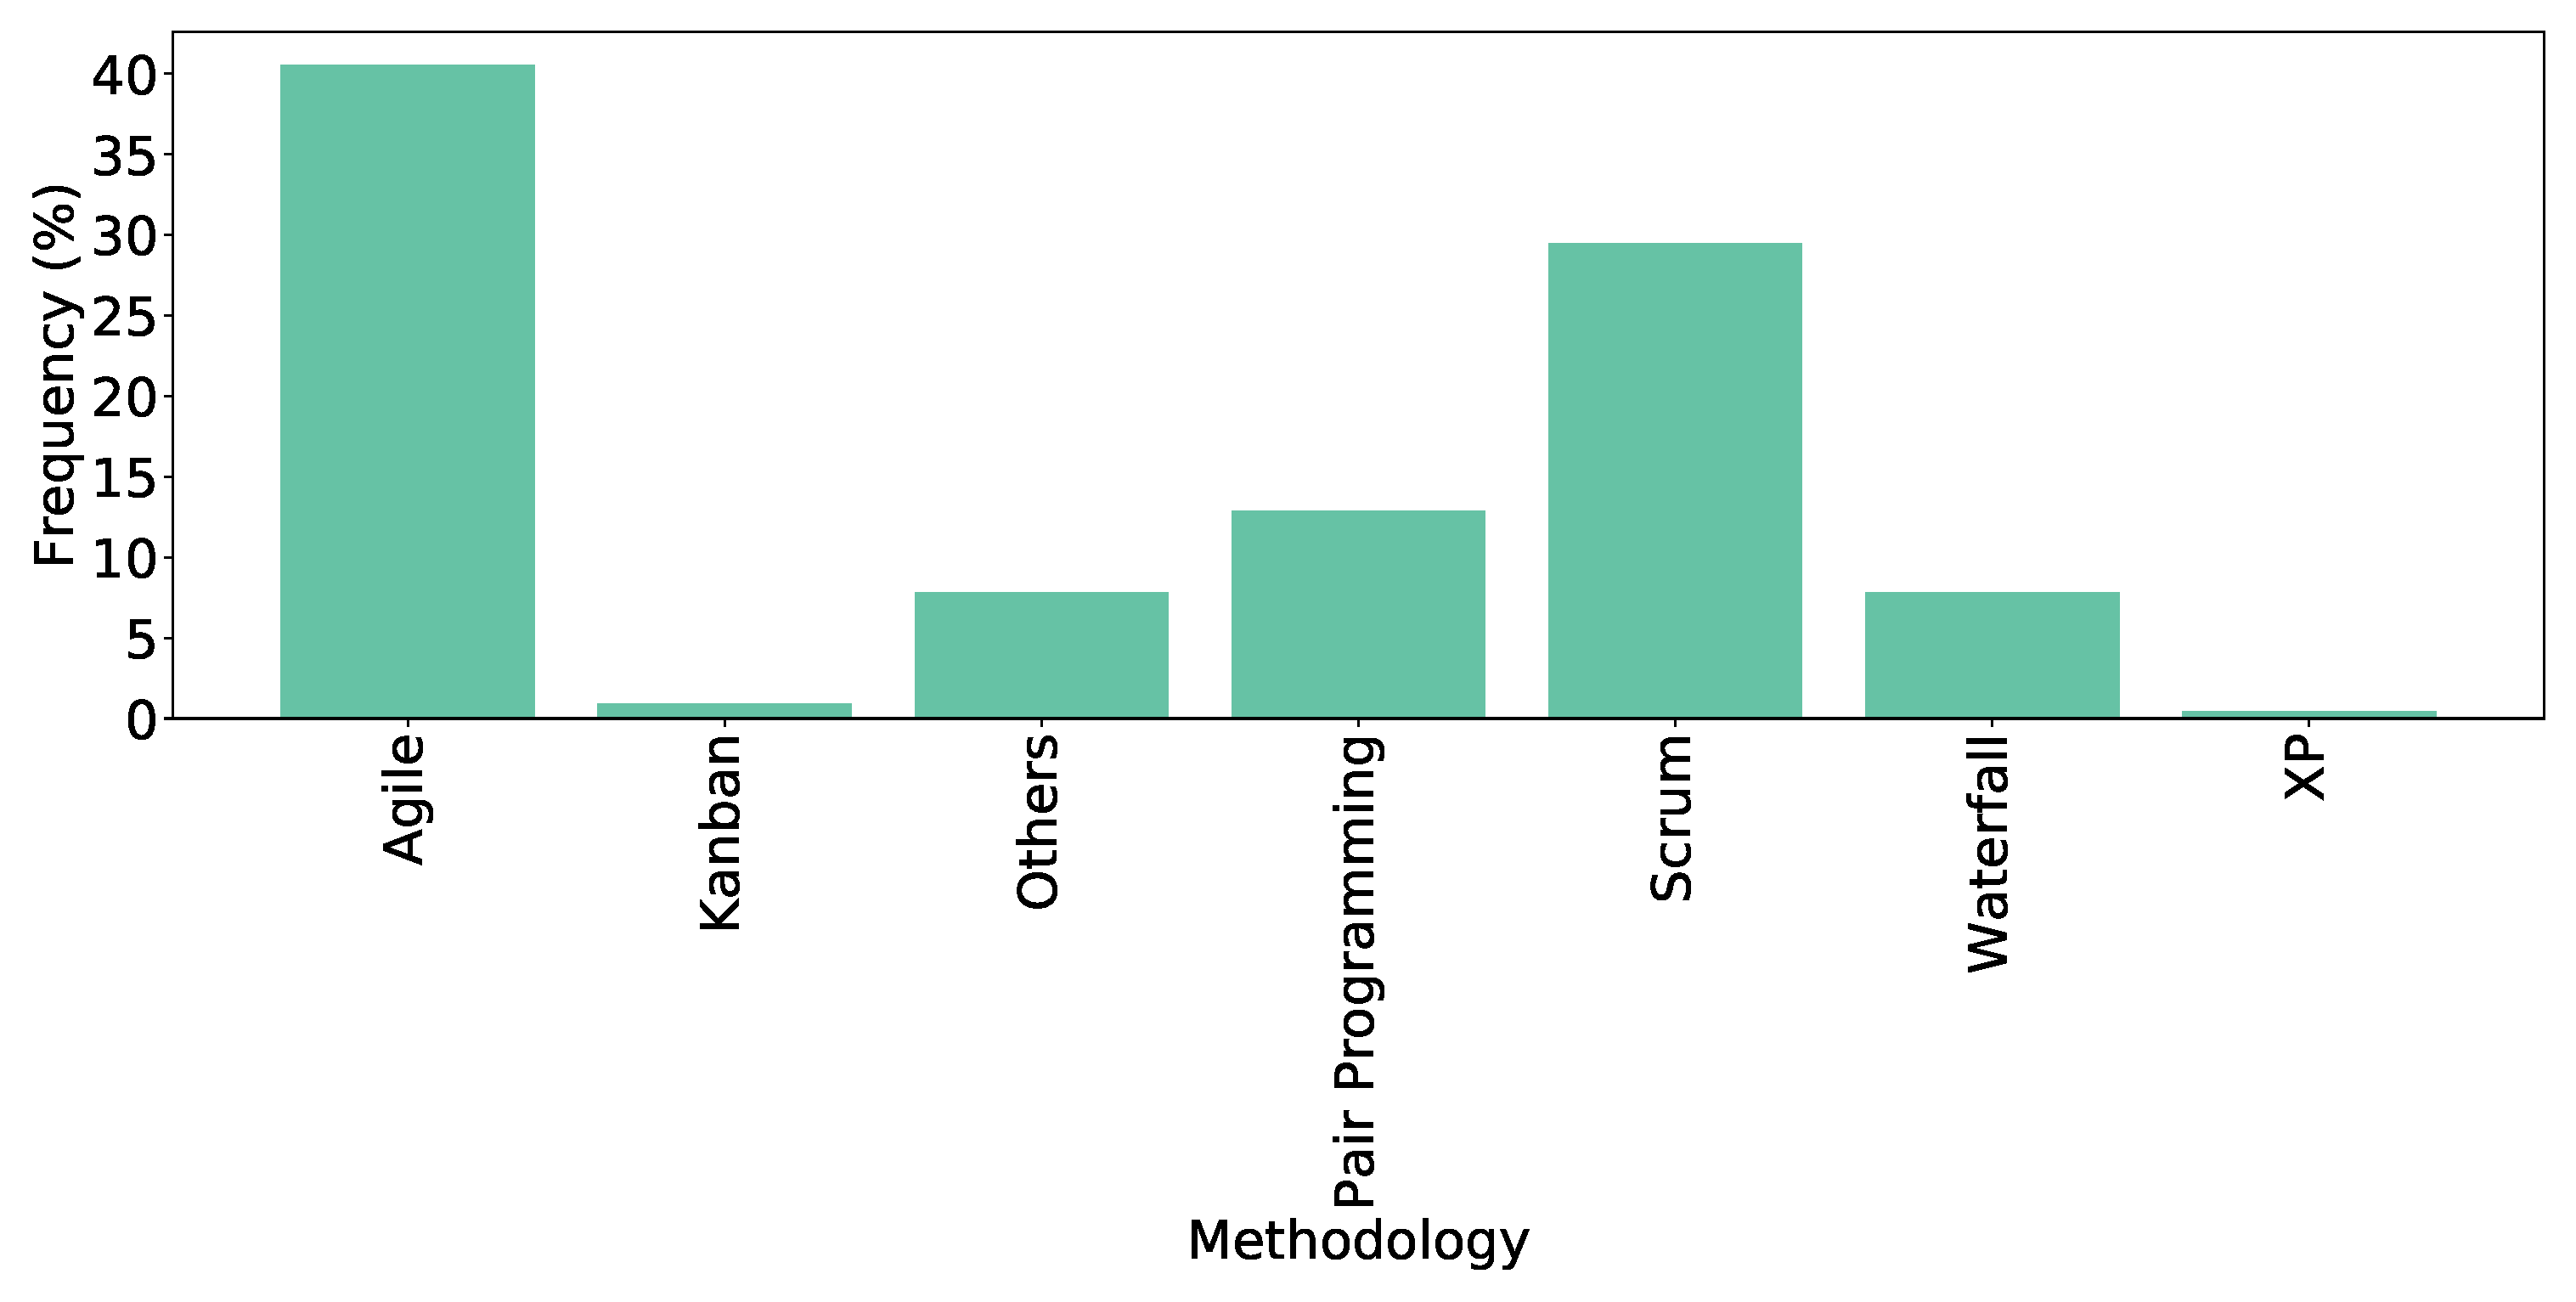
\includegraphics[width=0.8\textwidth]{Figures/Respondents_Methodology}
  \caption{Software development methodologies}
  \label{fig:methodologies}
\end{figure}

\subsubsection{Requirements Gathering}
The most critical activity that always arises during software development is the collecting requirement of the proposed system. According to \ref{fig:requirements}, using plain text (44\%) and story board (41\%) are the most widely used requirements gathering. This result is similar with the survey of Vonken et al. \cite{Vonken2012}. From their study we can find that the textual description of specifying requirements is a firm favourite in Netherlands. The other requirements gathering usage rates are: Use case (36\%), GUI prototype (35\%), grooming session (30\%) etc. This is an important finding that requires further analysis for causes and to analyze the potential effects of not documenting requirements.
\begin{figure}[htbp]
\centering
  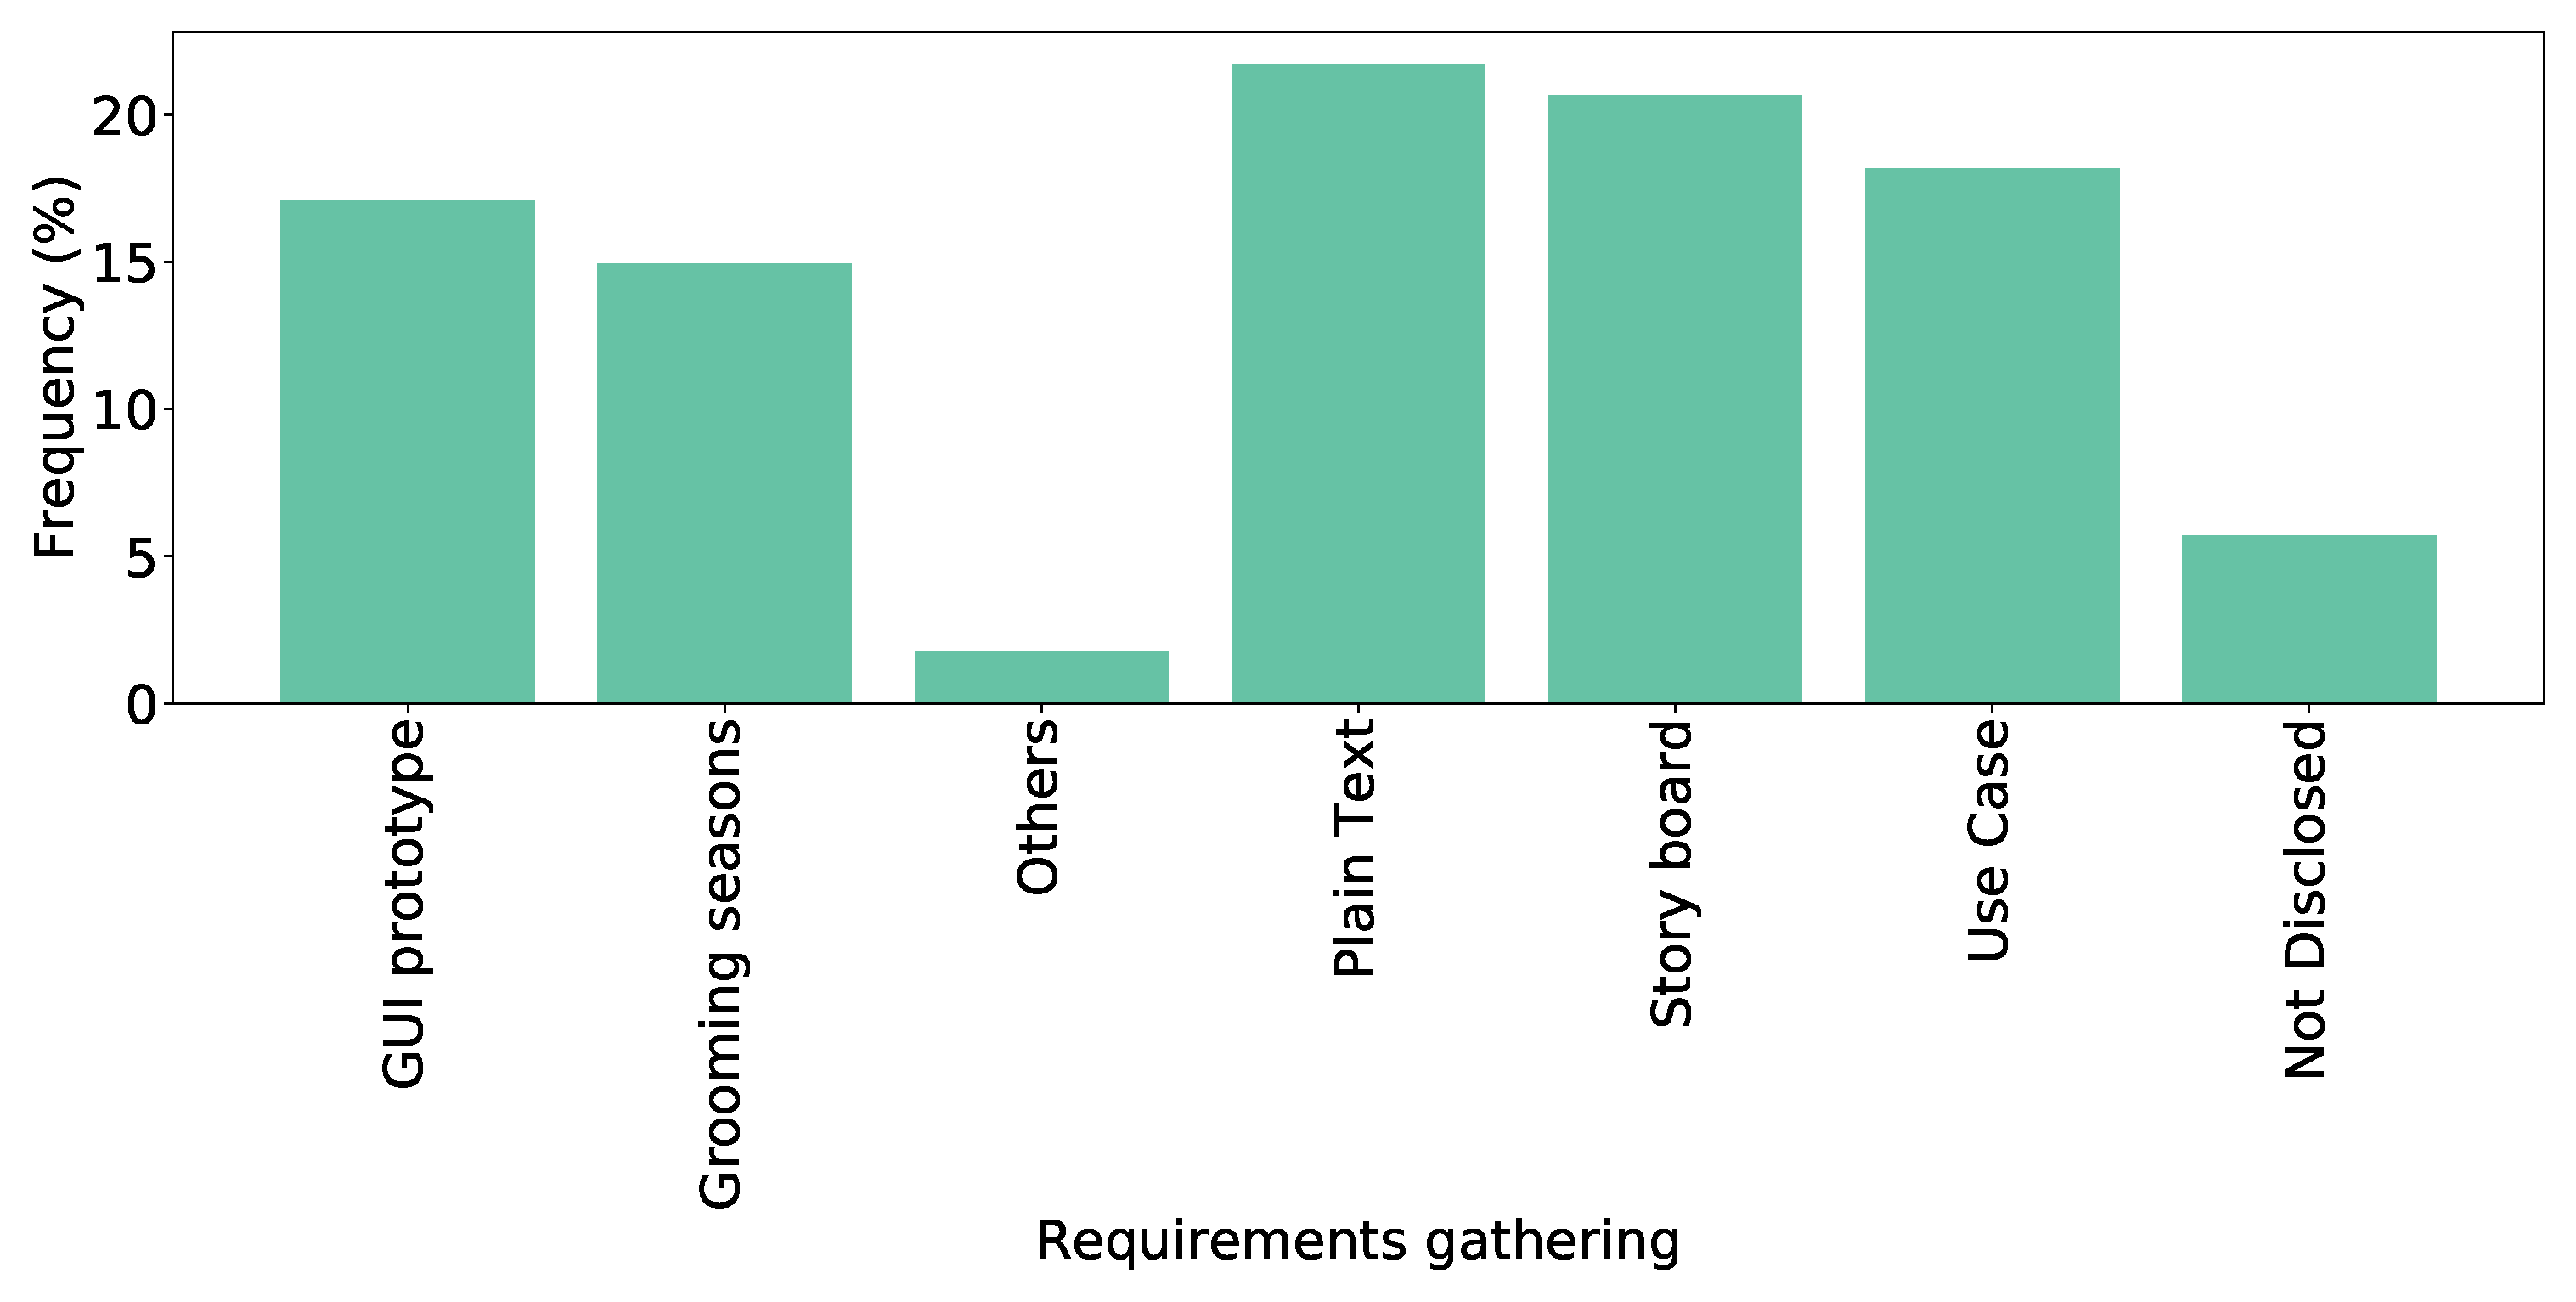
\includegraphics[width=0.8\textwidth]{Figures/Requirements_Gathering}
  \caption{Requirements gathering}
  \label{fig:requirements}
\end{figure}

\subsubsection{Development activities timeline}
In this section participants were asked about the most time consuming software developing activities they had spend. As we see in \ref{fig:activities}, most of the time spent in implementation stage according to 65\% our respondents and requirement analysis stage requires second most according to 45\% response. The other usages are: Program design (37\%), project planning (30\%), testing (19\%), maintenance (17\%) etc. According to study \cite{Wang2018}, most time was spent on implementation and coding and relatively less time was spent on maintenance in Bangladesh and New Zealand. But requirement analysis, the activity, requires the second most time to spend in Bangladesh where in New Zealand, it is testing (36\%) practices.

\begin{figure}[htbp]
\centering
  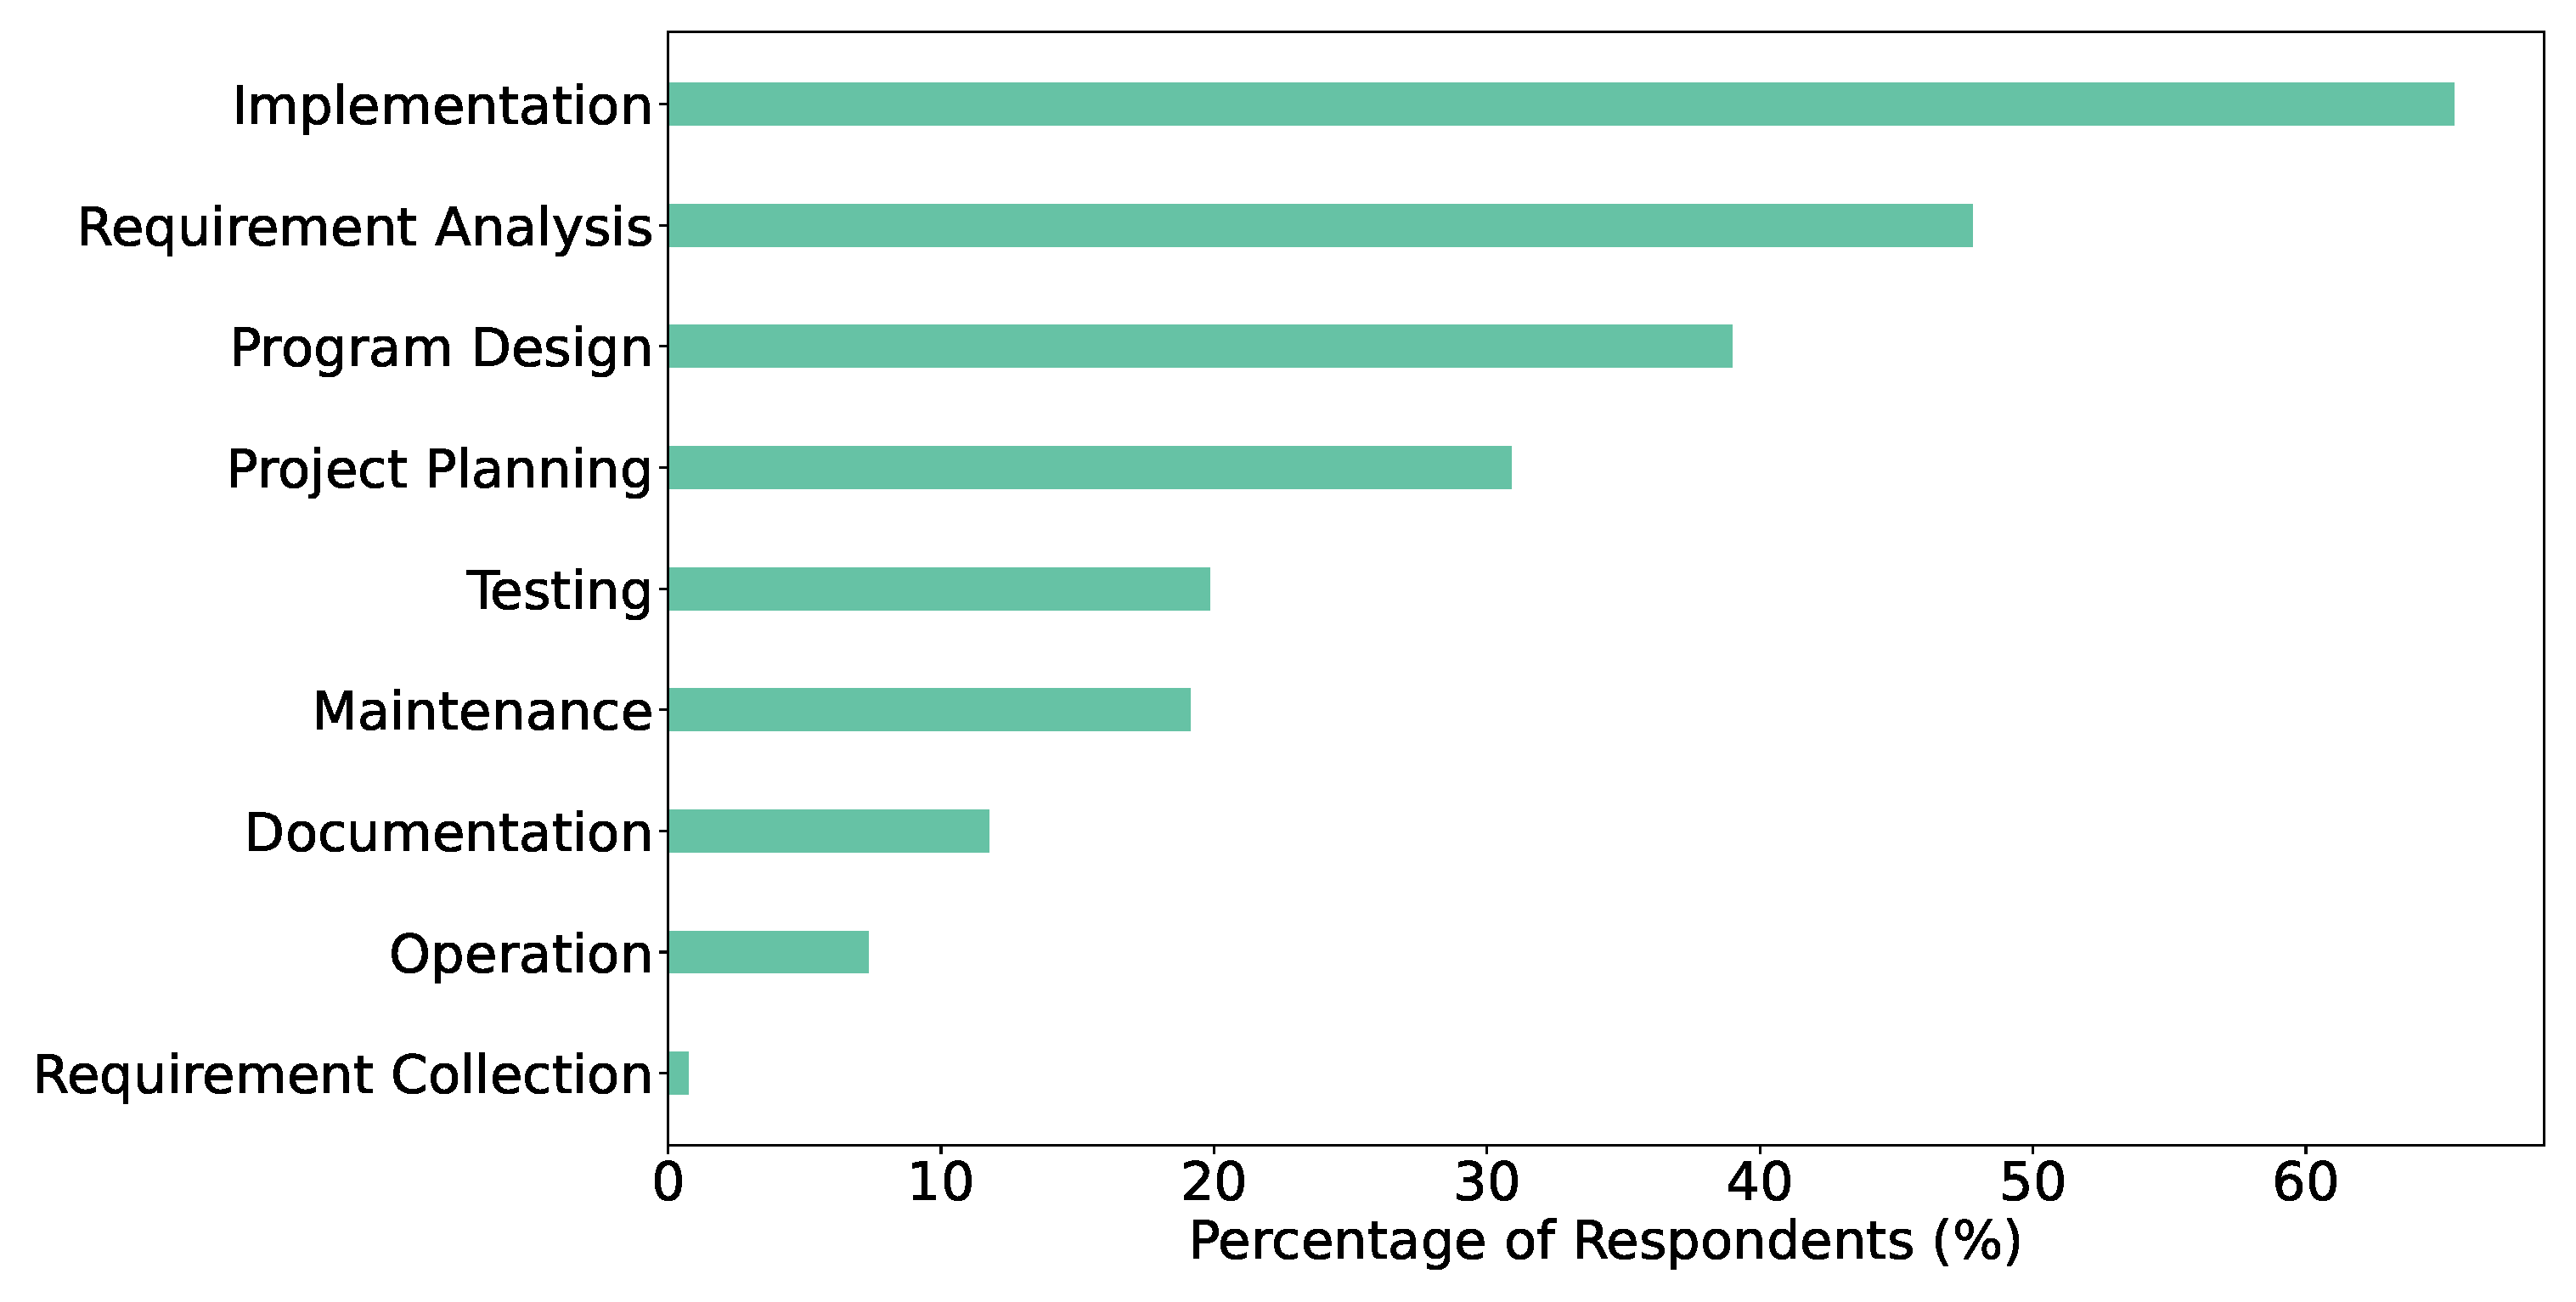
\includegraphics[width=0.8\textwidth]{Figures/Respondents_Activities}
  \caption{Software development activities}
  \label{fig:activities}
\end{figure}

